Terminal descent takes place in the following sequence, depicted schematically in Figure \ref{fig:tdseq}.
\begin{enumerate}
\item The rigid heat shield, joined in the middle by a bolt-and-nut assembly, is separated by redundant pyrotechnic cutters. The two halves are held fixed by locking actuators to prevent interference with exhaust flow and inflatable.
\item At this altitude, retro-propulsion is activated and the thruster provides the decelerating force in combination with the inflated aeroshell.
\item At an altitude of 50 [$m$], struts are partially deployed from their stowed position such that the pads rest above the inflatable. At the same time, the vent in the inflation system is opened and inflatable bladders deflate. Upon full deflation, measured by pressure transducers in the inflation system, the struts deploy further such that the pads are level with but below the thruster nozzle exit and achieve a roughly 90 [$deg$] inflatable half-cone angle.
\item The thruster is then deactivated and the crew capsule lands on the inflatable, on which the landing gear pads rest.
\end{enumerate}
\begin{figure}[h]
	\centering
	\begin{subfigure}[b]{0.44\textwidth}
		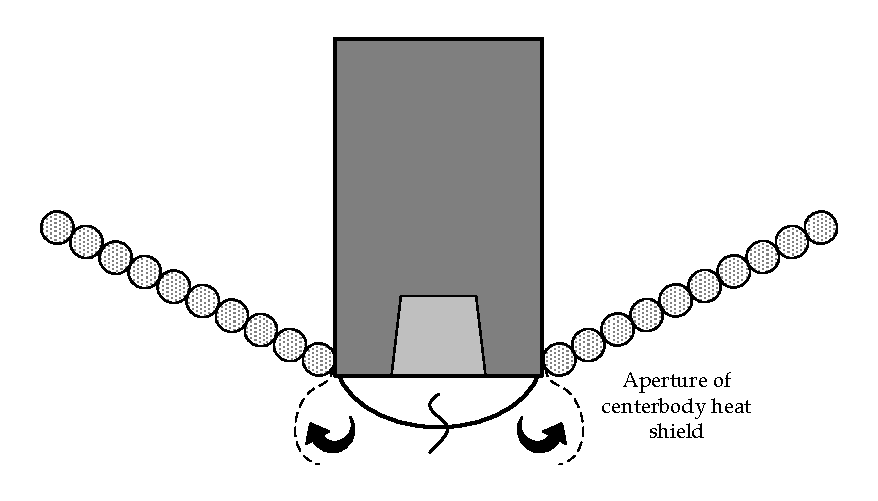
\includegraphics[width=0.96\textwidth]{./Figure/CrewModule/TDa.pdf}
		\caption{Retro-propulsion activation}
		\label{fig:rot}
	\end{subfigure}
		\begin{subfigure}[b]{0.55\textwidth}
		\centering
			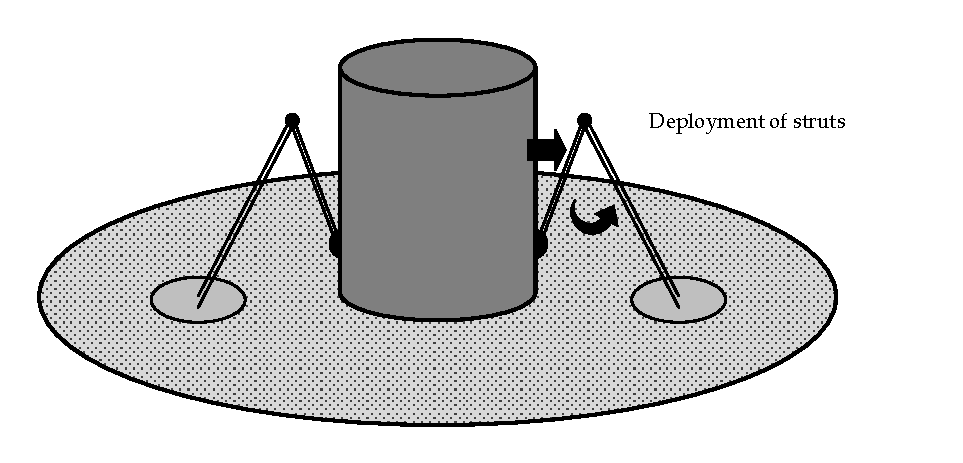
\includegraphics[width=0.96\textwidth]{./Figure/CrewModule/TDc.pdf}
			\caption{Strut deployment}
			\label{fig:hinge}
		\end{subfigure}
	\begin{subfigure}[b]{0.54\textwidth}
		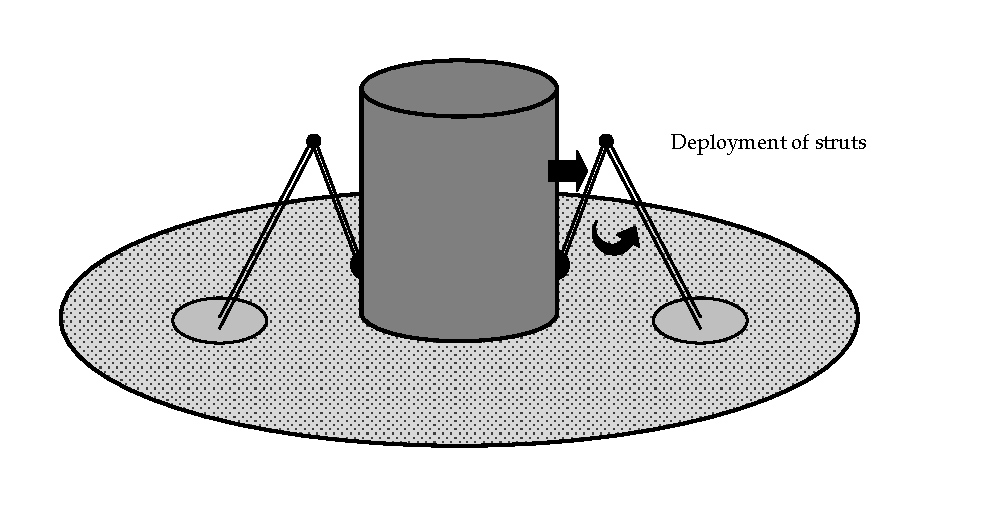
\includegraphics[width=0.96\textwidth]{./Figure/CrewModule/TDb.pdf}
		\vspace{-4.5mm}
		\caption{Decelerator deflation}
		\label{fig:fold}
	\end{subfigure}
		\caption{Terminal descent activity sequence}
	\label{fig:tdseq}
\end{figure}


Retro-propulsion is used for the beneficial aerodynamic interaction with a \gls{hiad} \cite{Korzun2009}, effecting a required specific impulse that is twice as low as otherwise. This effects a smaller propellant mass required. The inflatable is not rejected, but rather deflated, because rejection would require a separation mechanism to prevent interference with the crew capsule. Deflation does induce, however, the risk that it is not performed reliably. In such a case, a risk mitigation plan could be deliberate puncturing of the inflatable bladder volumes in order to deflate it.


The terminal descent system, as described in Section \ref{sec:terminal}, consists of the thruster system that decelerates the spacecraft from Mach 5 at 10 [km] height to zero velocity at a height of 0 [km]. The thruster should be placed in the centerbody and pointed in the forward direction, such that the positive interaction between aerodynamics and the thruster plume is made use of. The total terminal descent mass, including thruster, fuel, landing gear and drogue parachute, is estimated to be approximately 1445 [kg].